\chapter{Analysis}
Before we move to the nuts and bolts of AlphaZero and our concrete implementation, we should establish a general understanding of the problem. That includes establishing the necessary theoretical background in artificial intelligence in general, as well as insight into the specialized knowledge such as deep reinforcement learning.

\section{Artificial intelligence}
% explain some of the history of AI:
% - what does it mean
% - little bit of history: focus on symbolic vs subsymbolic

\subsection{Rational agent}
Stemming from the latin word \textit{agere} meaning "to act", an agent is something that acts. As we expect our agent to take sensible or intelligent actions we further qualify this definition by calling it rational. This means that it acts so as
\begin{quote}
    to achieve the best outcome or, when there is uncertainty, the best expected outcome.
\end{quote} \cite[p. 36]{russell_artificial_2021}

The agent exists in an environment which it percieves through sensors and it acts takes actions through its actuators. We refer to the content of  the sensors output for one observation as \textit{percept}. The cat uses eyes, ears and other sensors to percieve the world and its legs, claws and so on to interact with the world. This forms a loop of observing, deliberating and finally taking an action, whereafter the agent oberserves again as depicted in figure \ref{agent-environment-loop}. Internally our agent has some an \textit{agent function} that takes the entire history of percepts observed and the built-in knowledge and maps it an action. A concrete implementation of this abstract function is called \textit{agent program}.

\begin{figure}
    \centering
    \includesvg[height=7cm]{agent_environment_loop.svg}
    \caption{The agent-environment interaction loop}
    \label{agent-environment-loop}
\end{figure}

The agent program might just be a simple tabular mapping from percepts to actions or could use a complex model of rules about the environment.

\section{Environment}

\subsection{Abalone rules}
Abalone is a fairly new game, that was devised in 1987 by Michel Lalet and Laurent Lévi. Nevertheless, with more than four million global sales it has established itself as a classic game \cite{noauthor_abalone_2020}. Abalone is a two-player game consisting of a hexagonal board with 61 fields and 14 marbles for black and white respectively.

The goal of the game is to push six of the opponent's marbles off the playing field. The game's starting position is depicted in figure \ref{basics} (a). One, two, or three adjacent marbles (of the player's own color) may be moved in any of the six possible directions during a player's turn. We differentiate between broadside or "side-step" moves and "in-line" moves, depending on how the chain of marbles moves relative to its direction, which is shown in figure \ref{basics} (b) and (c).

\begin{figure}[!h]
    \centering
    \subfloat[Starting position]{
        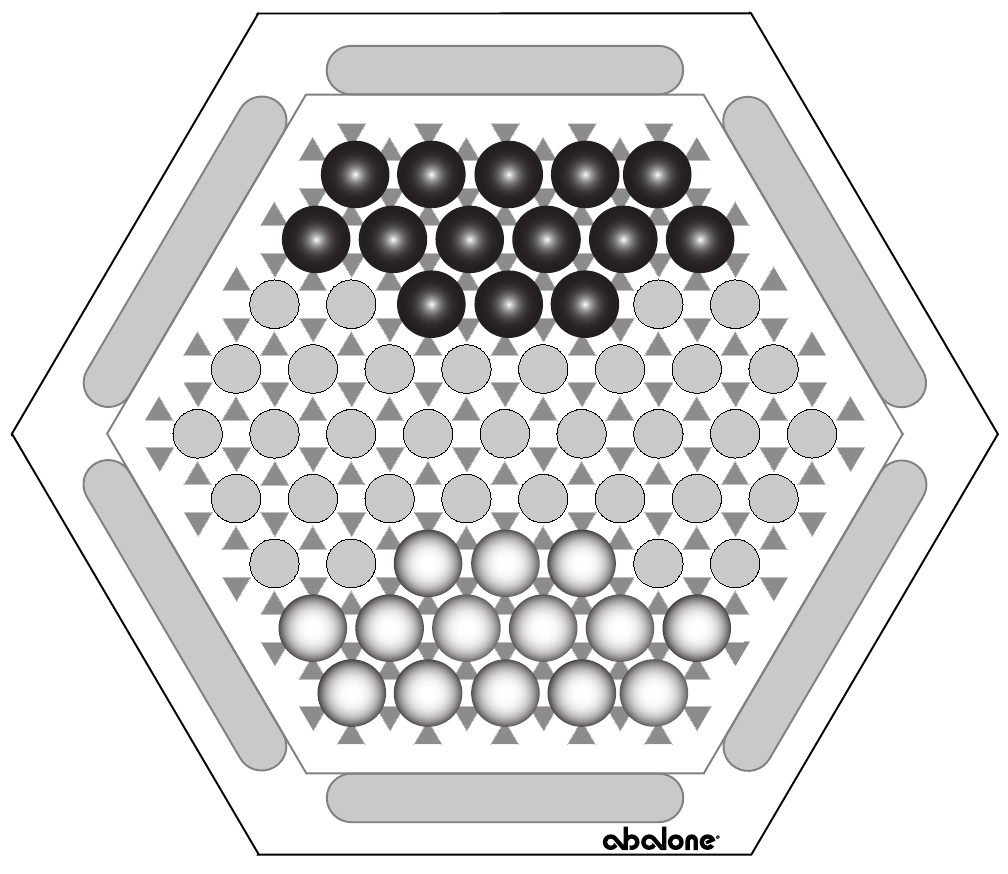
\includegraphics[width=3cm, keepaspectratio]{rules_starting_position.png}
    }
    \hfill
    \subfloat["In-line" moves]{
        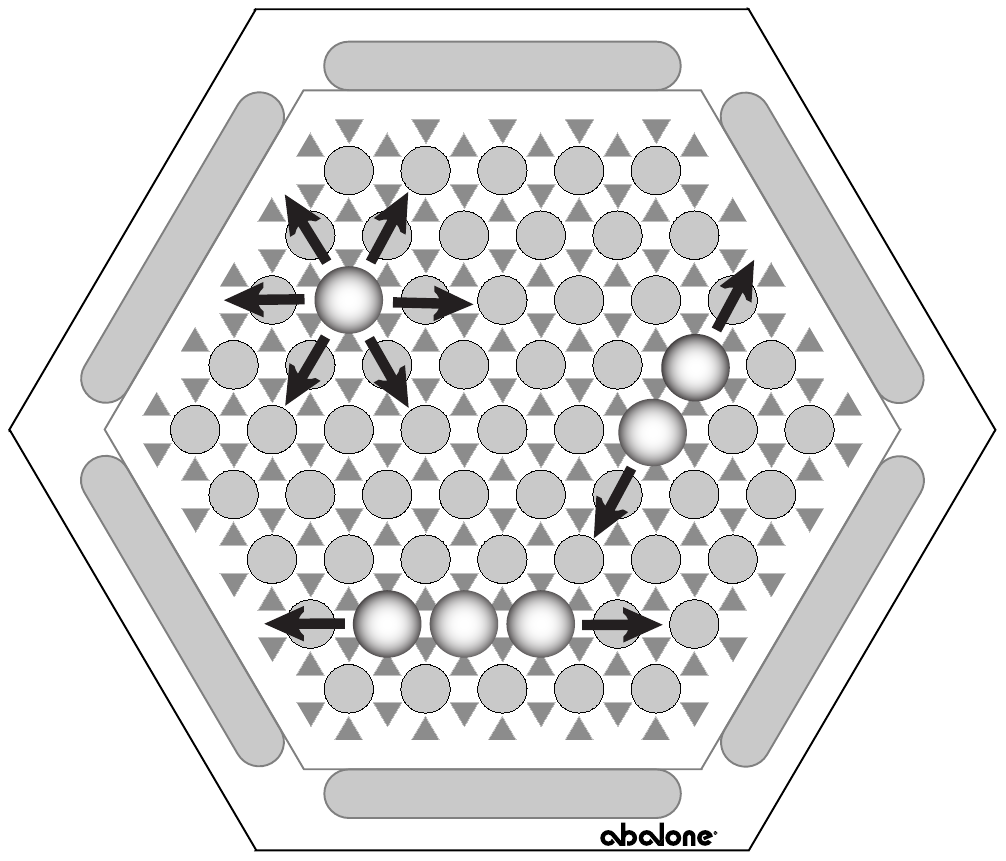
\includegraphics[width=3cm, keepaspectratio]{rules_inline_move.png}
    }
    \hfill
    \subfloat["Side-step" moves]{
        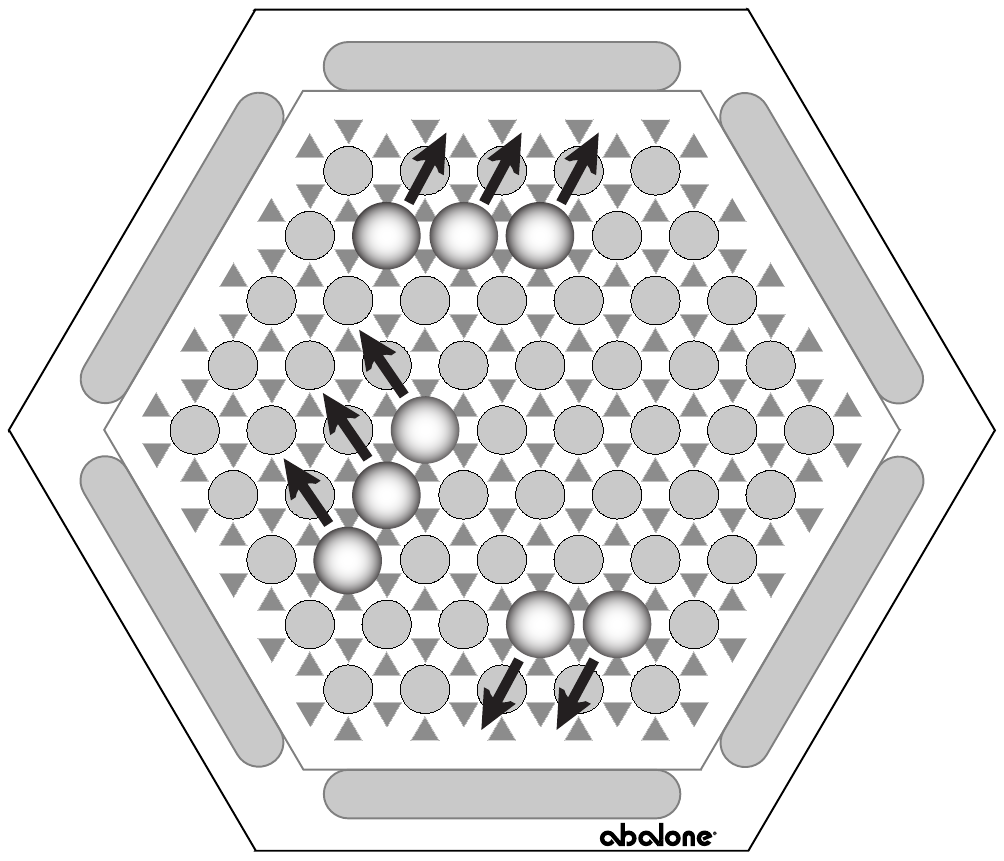
\includegraphics[width=3cm, keepaspectratio]{rules_side_step_move.png}
    }
    \caption{Basic moves \cite{abalone_sa_abalone_nodate}}
    \label{basics}
\end{figure}

A move pushing the opponent's marbles is called "sumito" and comes in three variations, as shown by figure \ref{sumito}. Essentially, the player has to push with superior numbers and the opponent's marbles can not be blocked. This is the game mechanic that allows for pushing the marbles out of the game and winning.

\begin{figure}[!h]
    \centering
    \subfloat["2-push-1" sumito]{
        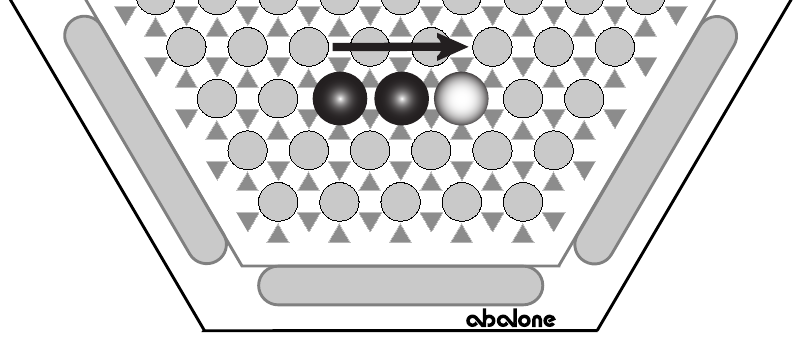
\includegraphics[width=3cm, keepaspectratio]{rules_2-push-1_sumito.png}
    }
    \hfill
    \subfloat["3-push-1" sumito]{
        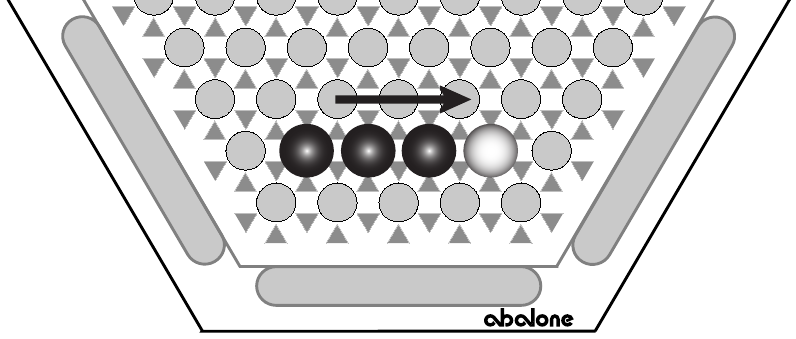
\includegraphics[width=3cm, keepaspectratio]{rules_3-push-1_sumito.png}
    }
    \hfill
    \subfloat["3-push-2" sumito]{
        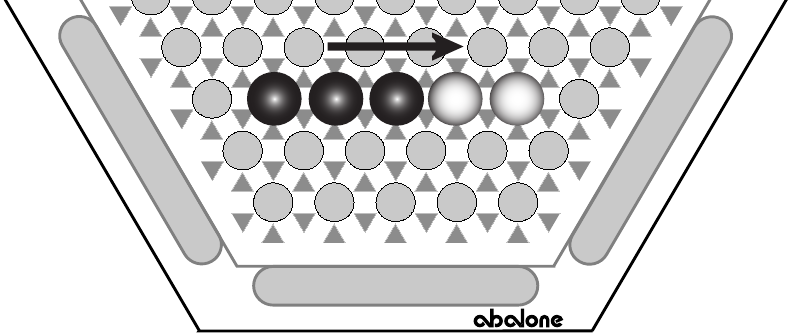
\includegraphics[width=3cm, keepaspectratio]{rules_3-push-2_sumito.png}
    }
    \caption{Sumito positions allow pushing the opponent's marbles \cite{abalone_sa_abalone_nodate}}
    \label{sumito}
\end{figure}

\subsection{Abalone complexity}

An important characteristic of a game environment is its complexity, which can be described in two relevant dimensions.

\paragraph{State space complexity}

The state space is the set of all possible states the agent can be in.\cite[p. 150]{russell_artificial_2021} For Abalone this means we have to consider all possible board configurations with different numbers of marbles present. Additionally, we would have to remove duplicates that arise from the symmetries of the board. In the case of abalone we have 6 rotations and 6 axes we can mirror the board on. The following formula gives us a good upper bound:

$$
    \sum_{k=8}^{14}\sum_{m=9}^{14}\frac{61!}{k!(61-k)!}\times\frac{(61-k)!}{m!((61-k)-m)!}
$$

\paragraph{Game tree complexity} The game tree defines the dependencies between board positions (nodes), moves (edges) and the resulting board positions. The number of nodes in a tree is given by:
$$
    b^d
$$
First we consider the branching factor $ b $, or the number of possible moves for any given state. We can only approximate this, as this number greatly varies between different states On average abalone has $ b = 60 $ possible moves per state as measured in figure \ref{branching_factor}. The depth $ d $ of the tree depends the number of turns per game. For some leaves this might be quite early, but as Abalone allows for actions to be taken repeatedly the height is potentiallly infinite. Looking at the average again a game takes in the region of $ d = 87 $ turns, giving us a total of $60^{87}$ nodes. \cite{lemmens_constructing_2005}

\begin{figure}
    \centering
    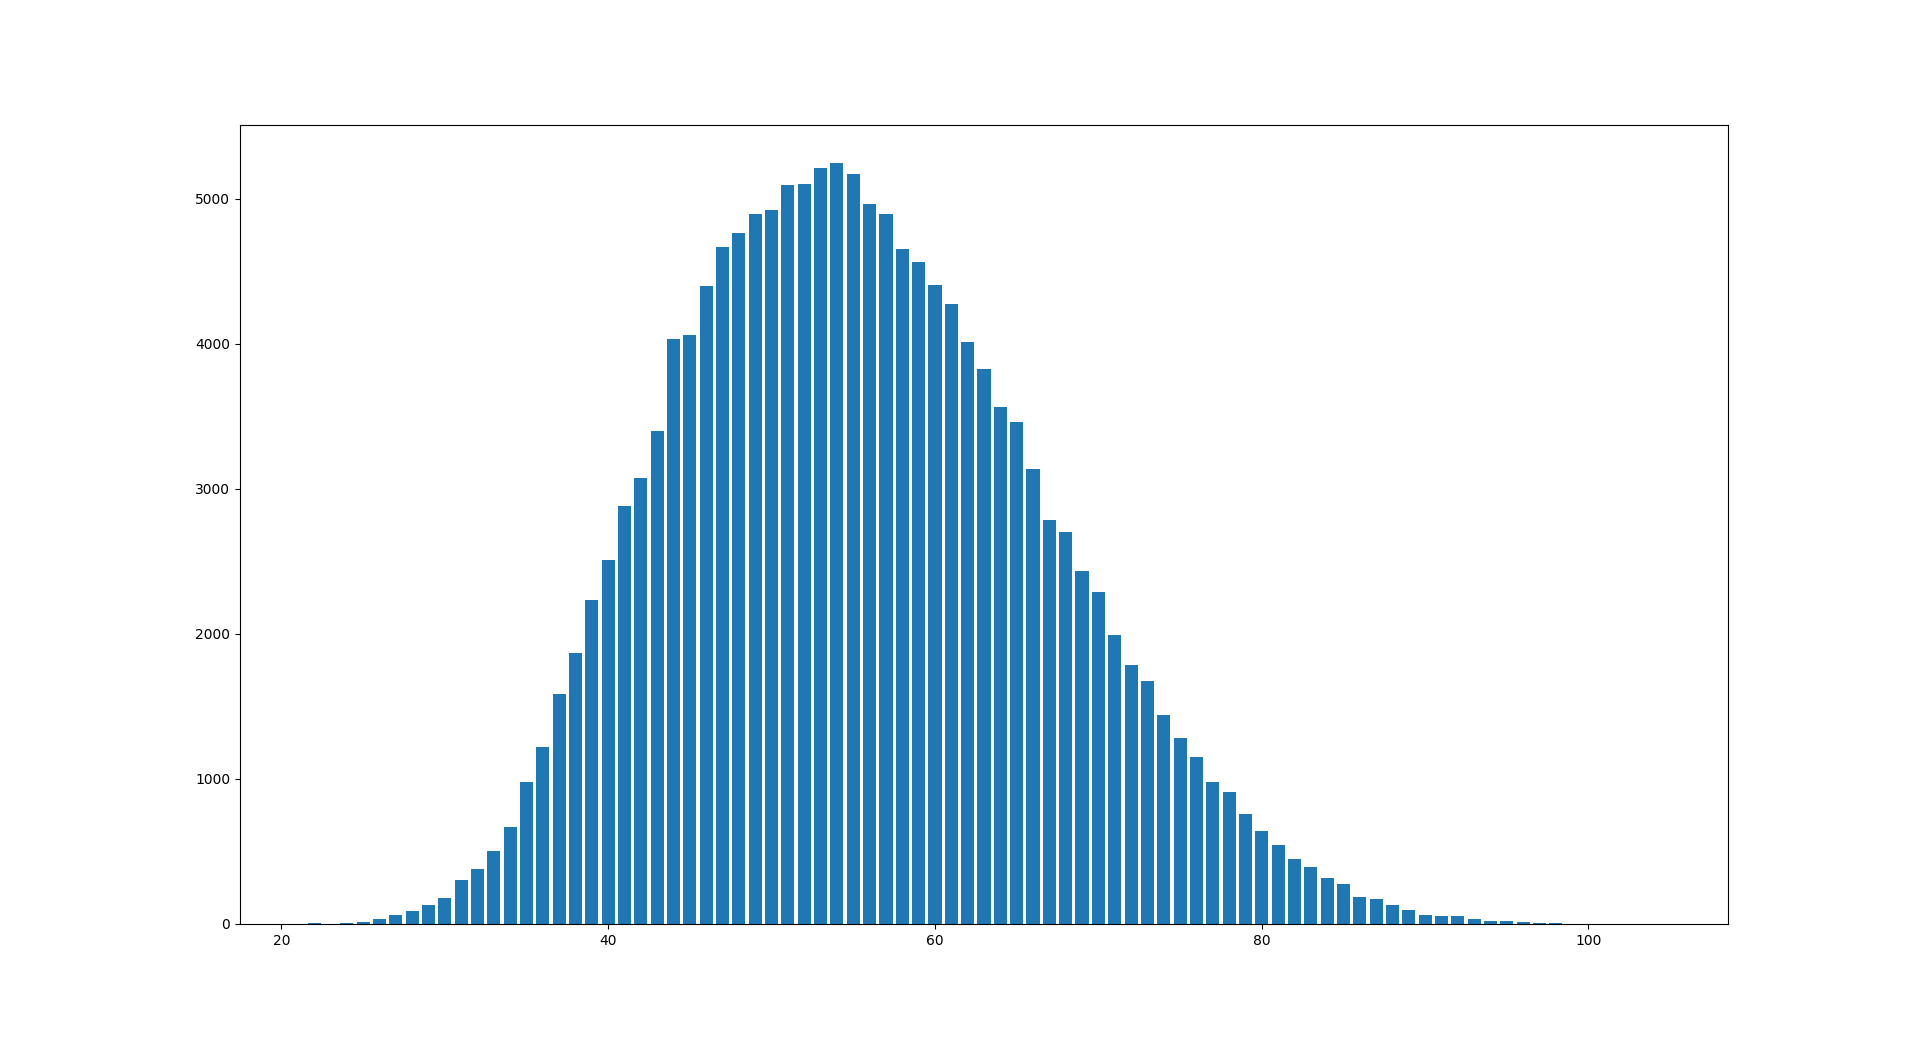
\includegraphics[width=7cm, keepaspectratio]{distribution_of_moves.png}
    \caption{Counts of moves available for random for random player in 5 games}
    \label{branching_factor}
\end{figure}

As those numbers in isolation are hard to grasp it is useful to put Abalone's complexity in relation with other popular games. Its state space complexity is on the same level as Reversi, whilst its game tree surpasses chess in complexity (c.f. table \ref{complexity_table})

\begin{table}
    \begin{center}
        \begin{tabular}{ | c | c | c | }
            \hline
            Game        & state-space complexity (log) & game-tree complexity (log) \\
            \hline
            Tic-tac-toe & 3                            & 5                          \\
            \hline
            Reversi     & 28                           & 58                         \\
            \hline
            Chess       & 46                           & 123                        \\
            \hline
            Abalone     & 24                           & 154                        \\
            \hline
            Go          & 172                          & 360                        \\
            \hline
        \end{tabular}
    \end{center}
    \caption{Abalone in comparison with other games \cite{chorus_implementing_2009}}
    \label{complexity_table}
\end{table}